Możliwość konstruowania układów warstwowych charakteryzujących się propagacją promieniowania elektromagnetycznego prostopadle do granicy warstw umożliwiła nie tylko konstrukcję supersoczewek, ale również elementów~o bardziej złożonej geometrii. Wykonując ścięcie pod pewnym kątem możemy warstwową supersoczewkę przekształcić~w element optyczny kształtem przypominający pryzmat, przykład prezentuje rysunek~\ref{fig:prism-schema}. Wykorzystując wielowarstwę~o efektywnych właściwościach zapewniających obrazowanie~z podfalową rozdzielczością, można taki układ wykorzystać do realizacji operacji rzutowania nie podlegającej klasycznemu ograniczeniu dyfrakcyjnemu~\cite{prism2010}. Uzyskując~w ten sposób obraz źródeł o charakterystyce podfalowej powiększony do rozmiarów umożliwiających obserwację za pomocą tradycyjnych mikroskopów. Możliwe jest również wykorzystanie superpryzmatu do zmniejszenia obrazu, dzięki czemu maska o rozmiarach większych od długości fali może posłużyć do wykonania litografii o rozmiarach podfalowych.

			\begin{figure}[tbH]
				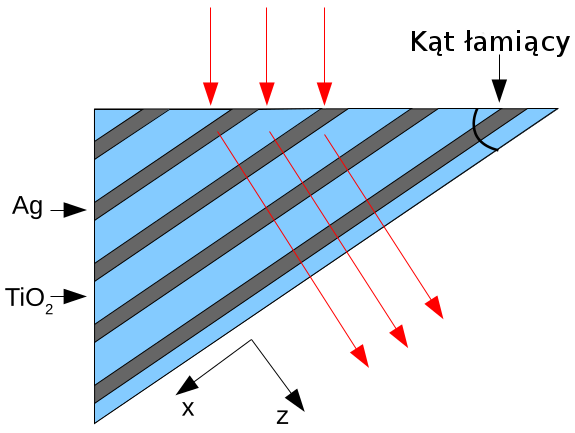
\includegraphics[width=\textwidth]{images/multilayer/prism.png}
				\caption{Schemat pryzmatu zbudowanego z metamateriału mogącego charakteryzować się kierunkową (prostopadłą do granicy warstw) propagacją fali elektromagnetycznej. Strzałkami schematycznie przedstawiono kierunek propagacji fali E-M.}
				\label{fig:prism-schema}
			\end{figure}


\begin{figure}[btH]
	\centering
			\begin{subfigure}{0.45\textwidth}
				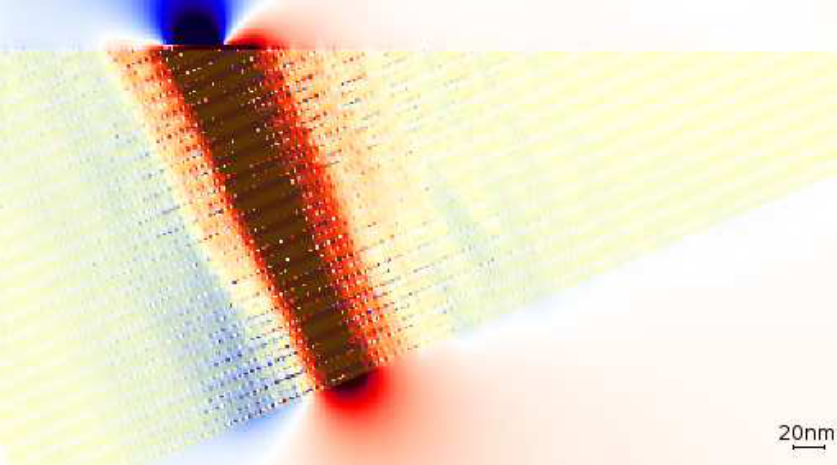
\includegraphics[width=\textwidth]{images/multilayer/prism04.png} \\
				\caption{Kąt łamiący 0.4 rad}
			\end{subfigure}
%			\begin{subfigure}{0.3\textwidth}
%				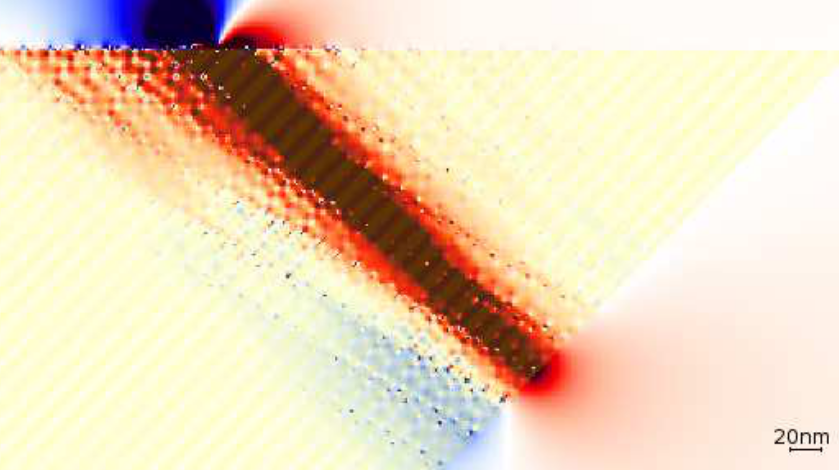
\includegraphics[width=\textwidth]{images/multilayer/prism08.png} \\
%				\caption{Kąt łamiący 0.8 rad}
%			\end{subfigure}
			\begin{subfigure}{0.45\textwidth}
				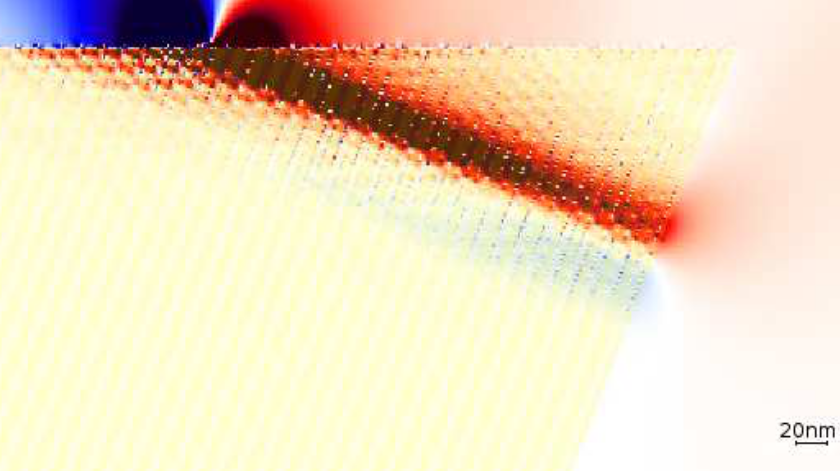
\includegraphics[width=\textwidth]{images/multilayer/prism12.png}\\
				\caption{Kąt łamiący 1.2 rad}
			\end{subfigure}
	\caption{Wynik symulacji metodą FDTD propagacji fali E-M przez superpryzmat. Pryzmat oświetlony został wiązką gaussowską o FWHM $90$~nm i długości fali $421$~nm~\cite{prism2010}}
\end{figure}

Wykorzystując dwa pryzmaty charakteryzujące się kierunkową propagacją światła, możemy realizować również inne przekształcenia geometryczne na dwuwymiarowych obrazach. Poprzez złożenie dwóch pryzmatów z rysunku \ref{fig:prism-schema} wzdłuż krawędzi równoległej do osi x, możemy uzyskać element wykonujący na obrazach o rozmiarach podfalowych operację obrotu. Składając w ten sposób dwa pryzmaty o kącie łamiącym równym 45$^\circ$ możemy zrealizować przesunięcie. Wykorzystując trzy pryzmaty możemy połączyć operację rzutowania i przesunięcia uzyskując efekt powiększenia lub pomniejszenia obrazu w jednym zintegrowanym mikroelemencie optycznym bez zmiany kierunku propagacji promieniowania E-M~\cite{Zhao:08}.

Ze względu na propagację światła wewnątrz MDM w określonym kierunku do projektowania układów, których elementy złożone są z omawianych ściętych wielowarstw metaliczno dielektrycznych wykorzystać można algorytm przypominający śledzenia promieni(ang. ray tracing). Kierunek promieni w wiązce wewnątrz wielowarstwy jest wymuszony  przez silnie anizotropową efektywną przenikalność elektryczną wielowarstwy, natomiast w przestrzeni swobodnej możemy o nim wnioskować na podstawie klasycznych praw dyfrakcji~\cite{pastuszczak2011slanted}.

\begin{figure}
	\centering
	\begin{subfigure}{.45\textwidth}
		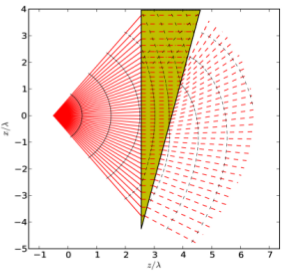
\includegraphics[width=\textwidth]{images/multilayer/prism-ray-tracing1.png}
	\end{subfigure}
	\begin{subfigure}{.45\textwidth}
		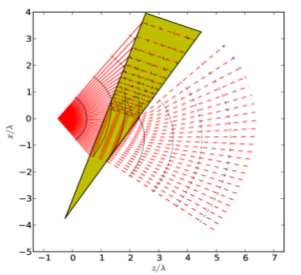
\includegraphics[width=\textwidth]{images/multilayer/prism-ray-tracing2.png}
	\end{subfigure}
	\caption{Przykłady algorytmu śledzenia promieni dla wiązki promieni przechodzącej przez pryzmat z metamateriału umożliwiającego obrazowanie podfalowe~\cite{pastuszczak2011slanted}} 
\end{figure}
